\documentclass[
	%parspace, % Add vertical space between paragraphs
	%noindent, % No indentation of first lines in each paragraph
	%nohyp, % No hyphenation of words
	%twoside, % Double sided format
	%draft, % Quicker draft compilation without rendering images
	%final, % Set final to hide todos
]{elteikthesis}[2021/09/20]

% The minted package is also supported for source highlighting
% See minted-intregration.tex for example
%\usepackage[newfloat]{minted}

% Document's metadata
\title{Dolgozat címe} % title
\date{2022} % year of defense

% Author's metadata
\author{Hallgató Hanga}
\degree{programtervező informatikus BSc}

% Superivsor(s)' metadata
\supervisor{Témavezető Tamás} % internal supervisor's name
\affiliation{egyetemi tanársegéd} % internal supervisor's affiliation
%\extsupervisor{Külső Kornél} % external supervisor's name
%\extaffiliation{informatikai igazgató} % external supervisor's affiliation

% University's metadata
\university{Eötvös Loránd Tudományegyetem} % university's name
\faculty{Informatikai Kar} % faculty's name
\department{Programozáselmélet és Szoftvertechnológiai\\ Tanszék} % department's name
\city{Budapest} % city
\logo{elte_cimer_szines} % logo

% Add bibliography file
\addbibresource{thesis.bib}

% The document
\begin{document}

% Set document language
\documentlang{hungarian}
%\documentlang{english}

% List of todos (not in the final document)
%\listoftodos[\todolabel]

% Title page (mandatory)
\maketitle
\topicdeclaration

% Table of contents (mandatory)
\tableofcontents
\cleardoublepage

% Main content
\chapter{Introduction}
\label{ch:intro}

Lorem ipsum dolor sit amet, consectetur adipiscing elit. In eu egestas mauris. Quisque nisl elit, varius in erat eu, dictum commodo lorem. Sed commodo libero et sem laoreet consectetur. Fusce ligula arcu, vestibulum et sodales vel, venenatis at velit \cite{dahl1972structured}. Aliquam erat volutpat. Proin condimentum accumsan velit id hendrerit. Cras egestas arcu quis felis placerat, ut sodales velit malesuada. Maecenas et turpis eu turpis placerat euismod.\footnote{Maecenas a urna viverra, scelerisque nibh ut, malesuada ex.}

Aliquam suscipit dignissim tempor. Praesent tortor libero, feugiat et tellus porttitor, malesuada eleifend felis. Orci varius natoque penatibus et magnis dis parturient montes, nascetur ridiculus mus \cite{cormen2009algorithms,krasner1988mvc}. Nullam eleifend imperdiet lorem, sit amet imperdiet metus pellentesque vitae. Donec nec ligula urna. Aliquam bibendum tempor diam, sed lacinia eros dapibus id. Donec sed vehicula turpis. Aliquam hendrerit sed nulla vitae convallis. Etiam libero quam, pharetra ac est nec, sodales placerat augue. \citeauthor{dijkstra1979goto} praesent eu consequat purus \cite{dijkstra1979goto}. 

\cleardoublepage

\chapter{Felhasználói dokumentáció}
\label{ch:user}


\section{Az alkalmazás célja}

Az alkalmazás célja, hogy a felhasználó segítségével membránrendszereket hozzon létre majd szimulálja számításaikat. A membránrendszer egy olyan biológiailag inspirált számítási modell, amely az eukarióta sejtek működését és felépítését követve evolúciós lépéseken keresztül történő információáramlást ír le membránok között. Minden membrán által körbezárt \textit{ún.} régió tartalmaz evolúciós szabályokat, amelyek nem változnak a membránrendszer működése közben. Az információt a rendszerben a régiókban található molekulák, \textit{ún.} objektumok hordozzák. Egy szabály csak akkor tud végbemenni, ha rendelkezésre állnak a szükséges objektumok kellő számban. Ilyen helyzetekben a szabályoknak végre is kell hajtódnia, tehát nem fordulhat elő, hogy minden objektum hozzáférhető, de nem kerül a szabály alkalmazásra. Egy evolúciós lépésben a maximális párhuzamosság elve érvényesül, azaz a szabályok véletszerűen kerülnek kiválasztása, egészen addig, amíg van alkalmazható szabály. Megadhatóak olyan speciális szamályok, amelyek alkalmazásának hatására egy membrán feloldódhat, ilyenkor a tartalma az őt körbevevő régióba kerül. A szabályok között prioritási sorrend is felállítható. A számítás legfontosabb tulajdonsága annak kimenete, amely általában a legkülső régión kívülre (azaz a környezetbe) kijutó objektumok számát jelenti.


\section{Hardver és szoftver követelmények}

A szoftver futtatásához Linux környezetre van szükség, amely támogatja az \verb|ELF| formátumú bináris állományok értelmezését. Ezen felül a futtatási környezetnek rendelkeznie kell \textit{Python interpreterrel}, illetve a \textit{Qt} keretrendszerhez való hozzáférés érdekében \verb|PySide6| modullal. Az utóbbi könnyen megtehető shell környezetben a \verb|pip install PySide6| paranccsal . A program teljes funkcionalitásának kihasználásához a felhasználó számítógépének a bemeneti perifériák közül egérrel és billentyűzettel kell rendelkeznie. A szoftver hardverigénye nem igényel részletesebb specifikációt.


\section{Futtatás}

Mivel a program futtatható állományban kerül a felhasználóhoz, ezért annak az indításhoz elegendő megnyitni a fájlt tartalmazó mappát, majd duplán kattintani a fájlt reprezentáló ikonra. Ugyanez parancssori környezetben is elvégezhető, ilyenkor a terminálban a megfelelő mappába való elnavigálás után a 
\verb|./MembraneSimulator| parancs megadásával futtatható a program.

\section{Grafikus felhasználói felület}

A felhasználó az alkalmazással a grafikus felhasználói felületen keresztül tud kommunikálni, amely a főablakot és az igény szerint megjelenő dialógusablakokat foglalja magába.

\subsection{Főablak}

\begin{figure}[H]
	\centering
	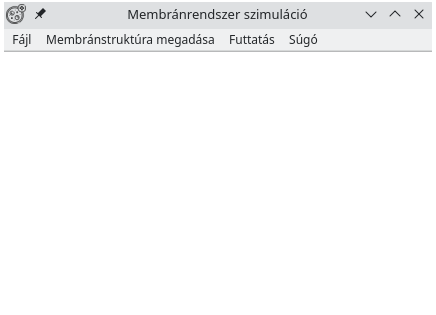
\includegraphics{main_window_empty.png}
	\caption{A főablak az alkalmazás megnyitásakor}
	\label{fig:main_window}
\end{figure}

A főablak az alkalmazás megnyitásakor még tartalmaz egyetlen grafikus elemet sem, viszont a menüsorban található menüpontok segítségével könnyedén változtatni lehet ezen. Ha a felhasználónak nincs korábbi tapasztala a program használatával, akkor érdemes a \textit{Súgó} menüpont kiválasztásával kezdenie, amelyről részletesen szó esik a \ref{help} fejezetben.

\subsection{Dialógusablakok}

A legfontosabb interakció a felhasználó és a szoftver között a dialógisablakokon keresztül történik.  

\subsubsection{Membránstruktúra megadása}\label{create_structure}

Egy membránrendszer megalkotásának kezdeti módja a struktúrájának megadásával kezdődik. Mivel egy membránrendszerben a membránok hierarchikusan helyezkednek el, ezért a teljes rétegződést nagyon jól lehet ábrázolni fa alakban, ahol mindenkinek a szülő csúcsa az őt legszűkebben tartalmazó régió. Ezzel egyenértékű az a felírás, amikor egyetlen karakterláncban fejezzük ki ugyanezt, azáltal, hogy egy régiót megfeleltetünk egy nyitó-csukó zárójelpárral. Ilyenkor a két zárójel között elhelyezett objektumok jelentik a régió tartalmát. Azonban nem csak objektumok, de más régiók is helyet kaphatnak, ezzel kifejezve azt, hogy a már említett régió közvetlen gyerekét szeretnénk megadni. 

\begin{figure}[H]
	\centering
	\subcaptionbox{Dialógusablak alapmodell létrehozásához}{
		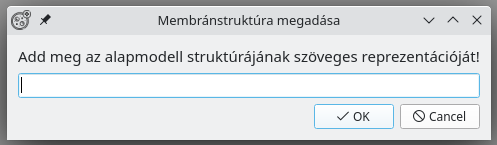
\includegraphics[width=0.4\linewidth]{structure_dialog_base_model.png}}
	\vspace{5pt}
	\subcaptionbox{Dialógusablak szimport-antiport rendszer létrehozásához}{
		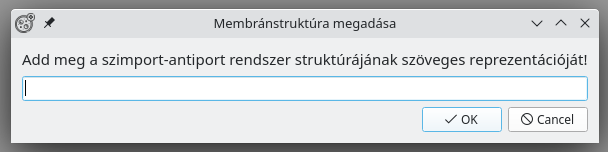
\includegraphics[width=0.45\linewidth]{structure_dialog_symport.png}}
	\caption{Dialógusablakok membránrendszer létrehozásához}
	\label{fig:create_system}
\end{figure}

A \ref{fig:create_system} ábra a különböző típusú membránrendszerek struktúrájának megadásához használt dialógusablakot mutatja. A megadott karakterláncban a régiók kezdetét és végét jelző zárójelpárok, illetve a bennük előforduló objektumok szerepelhetnek.
A helyes formátum feltétele, hogy a zárójelpárok karakterein és az szimport-antiport rendszereknél a kimeneti régió jelzésére használt speciális \textit{\#} karakteren kívül csak az angol ábécé kisbetűi szerepelhetnek a bemenetben, illetve annak meg kell felelnie a helyes zárójelezés szabályainak. Ezt azt jelenti, hogy nem lehetnek átfedések régiók között, azaz olyan karakterláncok, amikor egy külső régió hamarabb kerül lezárásra, mint bármelyik benne lévő régió. Ha ezen feltételeknek megfelel a felhasználó által megadott karakterlánc, akkor a főablak teljes területét lefedő vásznon megjelenik a létrehozott membránrendszer.

Ha a megadott karakterlánc nem a megfelelő formátumú, akkor a felhasználó figyelmeztetésére egy hibaüzenet jelenik meg a képernyőn. 

\subsubsection{Objektumok módosítása}

Miután a felhasználó megkonstruálta a membránrendszer szerkezetét, utána lehetősége nyílik arra, hogy az egyes régióinak tartalmát szerkessze. Mivel minden egyes régióhoz tartozhatnak objektumok és szabályok is egyaránt, ezért ezek módosítása közös dialógusablakban hajtható végre. A dialógusablak megjelenése a szerkeszteni kívánt régió által lefedett területre történő dupla kattintással kezdeményezhető. 

\begin{figure}[H]
	\centering
	\scalebox{0.8}[0.8]{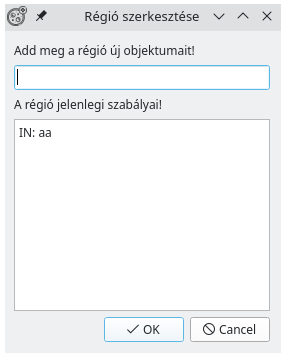
\includegraphics{rule_and_object_edit.png}}
	\caption{Dialógusablak egy régió tartalmának szerkesztéséhez}
	\label{fig:obj_edit}
\end{figure}

A régió objektumai közé tetszőleges számban írható a szóköz, mint elválasztó karakter, amely nem kerül figyelembevételre a régió új objektumainak feldolgozásakor. A megengedett karakterek ezen felül továbbra is az angol ábécé kisbetűi. Ha az adott régió a dialógusablak megnyitásakor már rendelkezik objektumokkal, akkor azok alapértelmezett szövegként fognak szerepelni a szövegdobozban. Tehát ha a régió szerkesztésekor az a felhasználó célja, hogy a kiválasztott régió tartalmát újabb objektumokkal egészítse ki, abban az esetben elegendő a hozzáadni kívánt karakterek begépelése.

\subsubsection{Szabályok módosítása}

A \ref{fig:create_system} segítségével alkotott membránrendszerek még nem fognak szabályokat tartalmazni, ám ezek nélkül nem beszélhetünk még szimulációról.  A szabályok fontos szerepet kapnak az információáramlás vezérlésében, hiszen a hatásukra tudnak objektumok átalakulni, be- és kivándorolni a régiók között. 

\begin{figure}[H]
	\centering
	\subcaptionbox{Régió szabályainak szerkesztése alapmodellben\label{fig:rule_edit_base}}{
		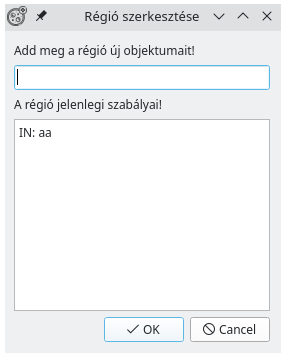
\includegraphics[width=0.45\linewidth]{rule_and_object_edit.png}}
	\vspace{5pt}
	\subcaptionbox{Régió szabályainak szerkesztése szimport-antiport rendszerben\label{fig:rule_edit_symport}}{
		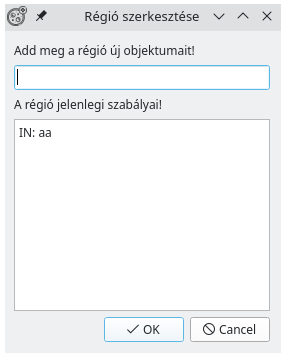
\includegraphics[width=0.45\linewidth]{rule_and_object_edit.png}}
	\caption{Membránrendszerek különböző formátumú szabályokkal}
	\label{fig:rule_edits}
\end{figure}

 A szabályok felépítése függ a membránrendszer típusától. Minden szabály megadása során először fel kell tüntetni, hogy mik azok az objektumok (olyankor ugyanolyan objektumból akár több is egyszerre), amelyek szükségesek a szabály alkalmazásához. 

Szimport-antiport rendszereknél ez a feltétel teljes mértékben elegendő ahhoz, hogy a szabály létrejöjjön, hiszen abban a modellben nincs lehetőség új objektumok létrehozására; a hangsúly inkább az objektumok régiók közötti mozgatására helyeződik. Ahogyan a \ref{fig:rule_edit_symport} alsó szövegdobozában is látható, szimport-antiport rendszerek esetében két különböző típusú szabály hozható létre. Az első a szimport szabály, amelynek két formája van. Az \textit{IN:} kezdetű szabály alkalmazása esetén a kijelölt objektumok a membránt körülvevő tartományból a jelenleg szerkesztés alatt álló tartományba vándorolnak; az \textit{OUT:} kezdetű szabálynál pedig a szerkesztés alatt álló régióból a membránt körülvevő tartományba kerülnek az objektumok. A másik típushoz az \textit{ún.} antiport szabályokat soroljuk, akkor egyszerre történik meg az előbbiekkel analóg módon be- és kivándorlás. A bevándorló objektumok előtt az \textit{IN:} prefix szerepel, a kivándorló objektumok pedig az \textit{OUT:} után találhatóak. Ezen két rész a karakterláncon belül felcserélhető, illetve köztük és az objektumok között tetszőleges számú szóköz karakter szerepelhet, amelyek a szabály megalkotásakor nem játszanak szerepet.

Ahogy a \ref{fig:rule_edit_base} ábra is mutatja, az alapmodell esetében a szabályok komplexebb felépítéssel rendelkezhetnek. Első nagy különbség, hogy ebben a modellben objektumok átalakulhatnak, illetve eltűnhetnek vagy megsokszorozódhatnak. Ebben a modellben a szabály alkalmazásához szükséges objektumokat a szabály \textit{bal oldalának} nevezzük. A szabály meghatározása ezen objektumok felírásával kezdődik. A szabály alkalmazásának köszönhetően létrejövő objektumok halmazát a nevezzük a szabály \textit{jobb oldalának}, amelyben az objektumok mozgásának figyelembevételével 3 csoportra bonthatunk:

\begin{compactenum}
	\item Kivándorló objektumok, amelyek a szülő régióba fognak jutni. Ha a legkülső régióban alkalmaztuk a szabályt, akkor az ilyen címkéjű objektumok a környezetbe kerülnek. A szabály megalkotásánál ezen objektumok elé az \textit{OUT:} prefix kerül.
	\item Bevándorló objektumok, amelyek véletlenszerűen valamelyik gyerek régióba fognak kerülni (az alapmodell ennél specifikusabban, címke alapján is megengedi az objektumok mozgását). A szöveges formátumban ezen objektumokat az \textit{IN:} szöveg előzi meg.
	\item Régión belül létrejövő objektumok, amelyek a szabályhoz tartozó régióba kerülnek. Ezen objektumok elé a karakterláncban a \textit{HERE:} kifejezés kell álljon.
\end{compactenum}
A szabály bal és jobb oldalát a \textit{->} szimbólumok választják el, amelyek együttesen egy nyilat reprezentálnak, annak kifejezésére, hogy a bal oldalt a jobb oldal objektumai ,,váljták fel''.
Tehát ekkor a \textit{ aa -> IN: bb OUT: cc HERE: dd} szöveghez tartozó alapmodellbeli szabály két \textit{a} objektumot igényel a végbemeneteléhez (amelyek felemésztődnek a reakció hatására), a régióból kivándorol két \textit{b} objektum, az egyik gyerek régióba bevándorol két \textit{c} objektum, illetve régión belül kialakul két új \textit{d} objektum.

Az alapmodell szabályai kiegészülhetnek többletjelentéssel is. Ebben a modellben ugyanis megengedett lehet egy régió felbomlása, amely egy vagy egyszerre több szabály előidézésére is bekövetkezhet. Ez a szándék jelezhető egy szabály konstruálásakor, ha a bal- és jobb oldalt elválasztó nyilat reprezentáló karakter után közvetlenül egy \textit{\#} karaktert ír a felhasználó. Ilyenkor a régió tartalma és gyerek régiói a szülő régiójába kerülnek.

% Struktúra gráfja
%\begin{tikzpicture}[node distance={20mm}, thick, main/.style = {draw, circle}] 
%\node[main] (1) {$1$}; 
%\node[main] (2) [below left of=1] {$2$}; 
%\node[main] (3) [below right of=1] {$3$}; 
%\node[main] (4) [below left of=2] {$4$}; 
%\node[main] (5) [below right of=2] {$5$}; 
%\draw (1) -- (2);
%\draw (1) -- (3); 
%\draw (2) -- (4); 
%\draw (2) -- (5); 
%\end{tikzpicture}


\subsubsection{Szimulációk számának megadása}

A korábbi dialógusablakok segítségével a felhasználó lehetőséget szerzett arra, hogy a teljes mértékben a saját elképzeléseinek megfelelő membránrendszer hozza létre és konfigurálja fel objektumokkal és szabályokkal. Ezek után már csak a rendszer számításának szimulálása van hátra. A szimulálás végrehajtására két módot biztosít az alkalmazás:

\begin{compactenum}
\item Teljes szimuláció futtatása párhuzamosan tetszőleges számú másolattal 
\item Egy szimulációs lépés az aktuális membránrendszeren
\end{compactenum}

Fontos megjegyezni, hogy a teljes szimuláció futtatásának kiválasztása esetén a képernyőn látható membránrendszer nem kerül szimulálásra, annak érdekében, hogy a szimulálni kívánt állapot megőrződjön, így utána változtatások nélkül kezdeményezhető a funkció megismétlése.

\begin{figure}[H]
	\centering
	\scalebox{1}[1]{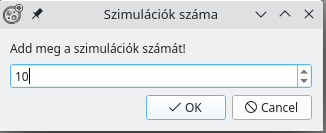
\includegraphics{num_of_simulation.png}}
	\caption{Dialógusablak a szimulációk számának kiválasztásához}
	\label{fig:num_of_sim}
\end{figure}

A szimuláció ismétléseinek számát egy olyan speciális szövegdobozzal lehet beállítani, amely bemenetként csak numerikus értékeket reprezentáló karaktereket fogad el. Alternatívaként a szövegdoboz jobb oldalán található nyilakkal is egyesével állítható az érték, amelynek alsó korlátja \textit{1}, felső korlátja pedig \textit{1000}.
 
\subsubsection{Mentés}
Miután a felhasználó kialakított egy olyan membránrendszert, amelyet szeretne elemezni vagy későbbi használat céljából megőrizni, az alkalmazás lehetőséget biztosít a jelenlegi állapot fájlba történő lementésére.

\begin{figure}[H]
	\centering
	\scalebox{0.5}[0.5]{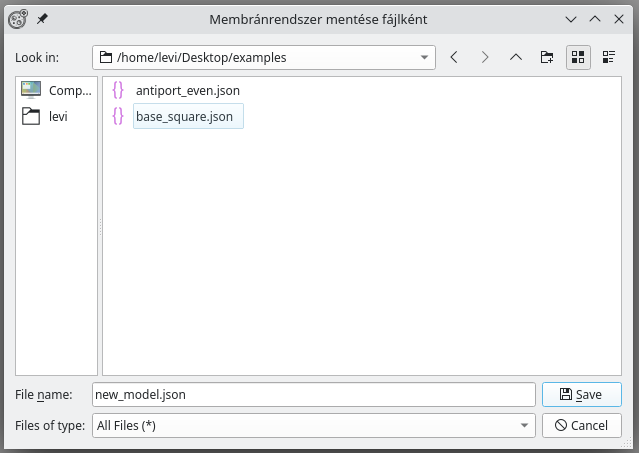
\includegraphics{save_system.png}}
	\caption{Dialógusablak a membránrendszer mentéséhez}
	\label{fig:save_system}
\end{figure}

A mentés folyamata a \textit{Mentés} gombra történő kattintással vagy a \verb| Ctrl+S| billentyűkombináció lenyomásával kezdeményezhető. A funkció kiválasztása után egy dialógusablak jelenik meg, amelyben a mentés helyére kell navigálnia a fájlrendszerben, majd a fájlnév megadása után az \textit{OK} gomb lenyomására létrejön a \textit{JSON} formátumú fájl a megadott útvonallal.

Mivel a \textit{JSON} formátum könnyen értelmezhető és szerkeszthető, ezért egy jártasabb felhasználója a programnak képes egy lementett membránrendszeren módosításokat végezni a megfelelő szerkesztésekkel. 


\begin{figure}[H]
	\centering
	\scalebox{0.4}[0.4]{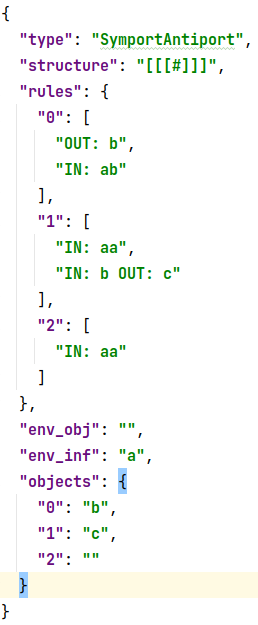
\includegraphics{saved_json.png}}
	\caption{Egy lementett membránrendszerhez tartozó JSON fájl  \protect\footnotemark}
	\label{fig:saved_json}
\end{figure}

\footnotetext{Az ábrán látható konfiguráció a páros számokat generáló szimport-antiport rendszerhez tartozik}

\subsubsection{Betöltés}

Az alkalmazás biztosítja lementett membránrendszerek betöltését, amelynek hatására betöltődik a kiválasztott fájlhoz tartozó állapot a grafikus felületre.
A betöltés nagyon hasonlóan működik a mentéshez, kezdeményezni a \textit{Betöltés} gombra történő kattintással vagy a \verb| Ctrl+O| billentyűkombináció lenyomásával lehetséges, mely után egy dialógusablak segítségével a felhasználó elnavigálhat a megnyitni kívánt fájlt tartalmazó mappához.

\begin{figure}[H]
	\centering
	\scalebox{0.5}[0.5]{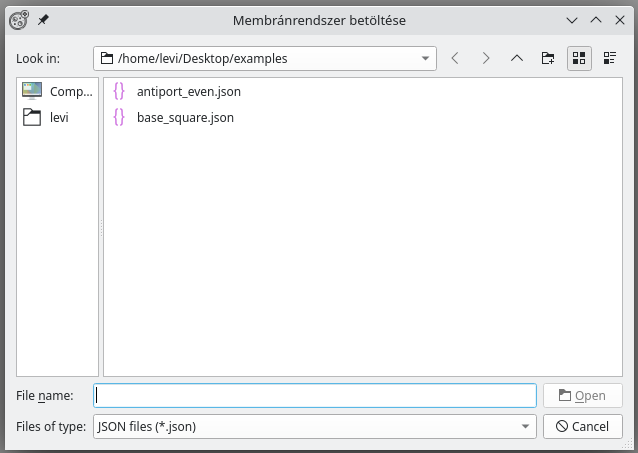
\includegraphics{load_system.png}}
	\caption{Dialógusablak egy membránrendszer betöltéséhez}
	\label{fig:load_system}
\end{figure}

\subsubsection{Eredményablak}

Miután a felhasználó létrehozott egy membránrendszert és szimulálta azt, nincs más hátra mint értesülnie annak eredményéről.  Ezt a funkciót látja el az eredményablak, amely a membránrendszer számításának befejeződése után automatikusan megjelenik és egy listában gyakoriság szerint növekvő sorrendbe rendezve jeleníti meg a különböző számítási eredményeket.

\begin{figure}[H]
	\centering
	\scalebox{0.5}[0.5]{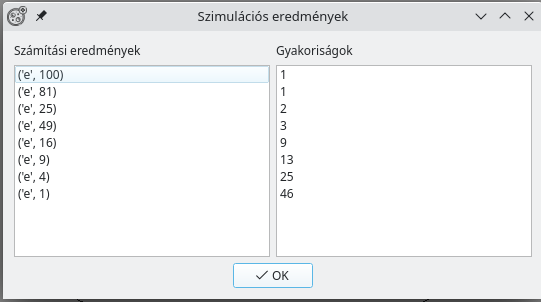
\includegraphics{results.png}}
	\caption{Szimulációs eredményeket kilistázó ablak}
	\label{fig:load_system}
\end{figure}

\section{Használati útmutató}\label{help}

A szoftver használata a membránrendszerek előzetes ismerete nélkül kriptikus tud lenni, ezért a felhasználó útbaigazítására és a szükséges jellemzőkkel kapcsolatos tudnivalók ismertetésére egy súgó funkció is megtalálható a menüsorban.

A használati útmutató a \textit{Markdown} formátumnak megfelelő formázásban jelenik meg, amely jól strukturált és könnyen olvasható. A tartalma fejezetekre van bontva, amelyek kitérnek a korábban említett dialógusablakok sajátosságaira, az objektumokkal és szabályokkal kapcsolatos elvárásokra és a szoftver helyes használatának módjára.
\cleardoublepage

\chapter{Fejlesztői dokumentáció}
\label{ch:impl}

A szoftver működésének részletezéséhez elengedhetetlen a membránrendszerek formális modelljének ismerete, hiszen ezen rendszerek sajátos viselkedése az architechturális kérdésekben döntő szerepet képez.

A teljes definíció előtt azonban érdemes még pár fogalmat bevezetni. Általánosan tehát egy olyan absztrakt számítási modell áll a szoftver központjában, amely egy biológiai sejthez hasonló felépítéssel rendelkezik, az egymásba ágyazott membránok régiókat különítenek el, amely régiókban különböző objektumok helyezkedhetnek el. A rendszerben az objektumokon felül szabályokat is rendelhetünk régiókhoz, ezen szabályok felelősek a membránrendszer állapotában végbemenő változásokért. A szabályokat a megfelelő feltételek teljesülése esetén kötelesek vagyunk alkalmazni, így egy evolúciós lépés a rendszer számításában addig tart, amíg van legalább egy akalmazható szabály. Érdemes már megjegyezni, hogy egy régió beazonosításához egy egyedi azonosítóra van szükség, illetve, hogy egy régiót könnyen azonosítani lehet az őt legszűkebben tartalmazó membránnal. Így természetes módon adódik, hogy a régiókat fa struktúrába tudjuk szervezni, amelyben minden egyes csúcs egy egyedi azonosítóval rendelkezik. Ezen fában a levelek az elemi membránokat reprezentálják, azaz azokat a régiókat, amelyeken belül nem helyezkedik el régió.  Ezen struktúra pedig nagyon könnyen megfeleltethető egy sztringnek.

A másik fontos tervezési szempont az objektumok reprezentálásához kapcsolódik. A membránrendszerek az egy régión belül megtalálható objektumok sokaságát ún. \textit{multihalmazokkal} reprezentálják, amelyben minden objektum rendelkezik egy multiplicitás értékkel, amely számosságát mutatja meg a régión belül. A multihalmaz teljeskörű értelmezéséhez pedig szükség van egy ábécére, amely a lehetségesen előforduló objektumok halmazát tartalmazza. Ezen multihalmazok felett pedig műveleteket kell tudni értelmezni, amelyek az evolúciós szabályok által megkövetelt funkciókat kell magukba foglalniuk. Mivel egy evolúciós szabály felhasználja az alkalmazásához szükséges objektumokat (azaz szintén egy multihalmazt), ezért szükség van egy olyan műveletre, amely a régióhoz tartozó multihalmazból eltávolítja a felhasznált objektumokat. Ezt a funkciót a multihalmazok közötti kivonás művelet fogja biztosítani. Ahhoz, hogy eldöntsük, hogy egy szabály alkalmazható-e egy régióban, elegendő megvizsgálni, hogy a régióhoz tartozó multihalmaz magába fogalalja-e a szabályhoz tartozó bal oldali objektumok multihalmazát. Erre a problémára a halmazok közötti részhalmaz reláció nyújt megoldást. Végül az újonnan keletkező objektumokból álló multihalmaz hozzáadását a régió jelenlegi tartalmához a multihalmazokra nézett unió művelettel lehet modellezni. 

Ezen megjegyzések után már bevezethetjük a membránrendszerek formális definícióját.

\section{Definíciók, formális modell}

\begin{definition}
Egy $\Pi = \langle O, \mu , \omega_1 , \dots , \omega_m, R_1 , \dots , R_m , i_o  \rangle$ rendezett $(2m + 3)$-ast membránrendszernek (alapmodell) nevezzük, ha

\begin{enumerate}
\item O egy objektumokból álló ábécé
\item $\mu$ egy \textit{m} membránból álló membránstruktúra. A régiók ekkor a $\{1,2, \dots, m\}$ elemeivel injektív módon vannak címkézve. Ilyenkor \textit{m}-et $\Pi$ fokának nevezzük.

\item  $\omega_1 , \dots , \omega_m$ O feletti multihalmazokat reprezentáló sztringek, amelyek rendre az $1, 2, \dots, m$ címkéjű régiókhoz vannak rendelve

\item $R_i, 1 \leq i \leq m \; \mu \; i$-edik membránjához rendelt O feletti \textit{evolúciós szabályok} véges halmaza. A szabályok $u \rightarrow v$ alakúak, ahol $u \in O^+, v \in (O \times TAR)^*$, ahol $TAR=\{here, out\} \cup \{ in_j | q \leq j \leq m \} $ Ha nem írjuk ki a $j$ indexet, akkor nemdeterminisztikusan történik régió kiválasztása

\item$ i_o \in \{1,2, \dots, m\}$ egy elemi membrán címkéje, amely a modell kimeneti membránja.
\end{enumerate}
\end{definition}

Az előbbi definícióban meghatározott membránrendszerre a dolgozatban alapmodellként fogok hivatkozni. Az alkalmazás az alapmodell esetén csak a nemdeterminisztikus $in$ címkét engedi meg a szabályoknál. Ennek oka, hogy a szöveges reprezentációban csak így garantálható az, hogy egy karakter egy objektumot reprezentál, bárhol is szerepeljen a sztringben, illetve a régiók kézzel történő felcímkézésére sincs ezáltal szükség, hiszen ez lenne az egyetlen művelet, amely explicit használja a címkéket. 

A számítás formalizálásához fontos bevezetni a konfiguráció fogalmát.
\begin{definition}\label{def:mem_sysm}
A $C = (w_1, \dots, w_m)  \; a  \; \Pi = \langle O, \mu , \omega_1 , \dots , \omega_m, R_1 , \dots , R_m , i_o  \rangle$ membránrendszer konfigurációja, ha $w_i \in O^*$ és $w_i$ az $i$-edik régióban lévő objektumokból álló multihalmaz sztring reprezentációja
\end{definition}

\begin{note}
Egy $C$ konfiguráció kezdőkonfiguráció, ha $ \; \forall 1 \leq i \leq m$ esetén $w_i = \omega_i$
\end{note}

\begin{definition}
A megállási konfiguráció olyan konfiguráció, amelyre nem lehet már evolúciós szabályt alkalmazni.
\end{definition}

\begin{definition}
Az egylépéses konfigurációátmenet $C_1 \Longrightarrow_\Pi C_2$, akkor ha $C_1$-ből egy evolúciós ütemben megkapható $C_2$ (a maximális párhuzamosság elvének megfelelve). 
\end{definition}

\begin{note}
Mivel a szabályok alkalmazása nemdeterminisztikus, ezért a konfigurációátmenet relációban egy $C_1$-hez több $C_2$ is létezhet.
\end{note}

\begin{definition}
A többlépéses konfigurációátmenet a $\Longrightarrow_\Pi$ reláció reflexív tranzitív lezártja. 
\end{definition}

A rendszer egy számítása alatt tehát a kezdőkonfigurációból egy megállási konfigurációba történő többlépéses konfigurációátmenet-sorozatot értünk.

\begin{note}
Ilyenkor a számítás eredményét többféleképpen definiálhatjuk. Alapértelmezetten a kimeneti régióban lévő objektumok számát jelenti. Az alkalmazás az alapmodell esetén ettől eltér és a környezetbe kijutó objektumok számát tekinti a számítás eredményének.
\end{note}

Létezik olyan kiterjesztése az \ref{def:mem_sysm} definíciónak, amelyben megengedünk olyan $u \rightarrow v \delta$ alakú szabályokat, ahol az $u \rightarrow v$ az eddigiekhez hasonló evolúciós szabály, a $\delta$ pedig egy speciális szimbólum, amely a membrán feloldódását jelzi a szabály alkalmazásának hatására. Tehát ha egy evolúciós lépésben alkalmazásra kerül egy ilyen speciális szabály, akkor az ütem végén a szabályhoz tartozó régió felbomlik, ilyenkor a benne lévő objektumok és membránok ( a szabályok nem) a membránt közvetlenül tartalmazó szülő régióba kerülnek. A legkülső régió sosem oldódhat fel. 

A másik kiterjesztés a szabályok feletti részberendezés lehetőségét adja meg, mely szerint ha $r_1$ és $r_2$ relációban állnak (amelyet jelölhetünk $r_1 < r_2$-vel), akkor csak abban az esetben alkalmazható az $r_1$ szabály, ha $r_2$ már nem alkalmazható az evolúciós lépésben.

A szoftver mindkét kiterjesztést alapértelmezetten támogatja, működésüket a későbbi fejezetekben részletesebben kifejtem.

Az alkalmazás az alapmodell mellett a szimport-antiport rendszerek szimulálását támogatja. 
Ebben a modellben az objektumok nem alakulhatnak át, csak a membránstruktúrán belül és a környezetbe vándorolhatnak. Az eddig definiált fogalmak a szimport-antiport rendszereknél is helyt állnak, egyedül a szabályok alakja és működéseigényel módosításokat. 
Ezen felül a szimport-antiport rendszerek környezete rendelkezhet az $O$ ábécé egy olyan speciális részhalmazával, amelyben előforduló objektumok korlátlanul rendelkezésre állnak az evolúciós lépések során.
Ennek megfelelően vezessük be az alábbi definíciót.

\begin{definition}
Egy $\Pi = \langle O, \mu , E, \omega_1 , \dots , \omega_m, R_1 , \dots , R_m , i_o  \rangle$ rendezett $(2m + 4)$-est szimport-antiport rendszernek nevezünk, ha

\begin{enumerate}
\item O egy objektumokból álló ábécé
\item $\mu$ egy \textit{m} membránból álló membránstruktúra. A régiók ekkor a $\{1,2, \dots, m\}$ elemeivel injektív módon vannak címkézve. Ilyenkor \textit{m}-et $\Pi$ fokának nevezzük.

\item  $\omega_1 , \dots , \omega_m$ O feletti multihalmazokat reprezentáló sztringek, amelyek rendre az $1, 2, \dots, m$ címkéjű régiókhoz vannak rendelve

\item $E \subset O$ a környezetben korlátlanul rendelkezésre álló objektumok halmaza

\item $R_i, 1 \leq i \leq m \; \mu \; i$-edik membránjához rendelt O feletti szimport/antiport szabályok véges halmaza

\item$ i_o \in \{1,2, \dots, m\}$ egy elemi membrán címkéje, amely a modell kimeneti membránja.
\end{enumerate}
\end{definition}

Ebben a modellben legyenek $x, y \in O^+$ objektumok multihalmazait reprezentáló sztringek. A velük alkotott szabályok az alábbi alakok egyikét ölthetik:

\begin{enumerate}
\item (x, in): Ilyenkor az x multihalmaz a membrán körül elhelyezkedő, őt legszűkebben tartalmazó régióból a membrán által határolt régióna vándorol
\item (x, out): Ilyenkor az x multihalmaz az őt tartalmazó régióból a membránt körülvevő régióba mozog
\item (x, in; y, out): Ilyenkor az x multihalmaz a membrán körül elhelyezkedő, őt legszűkebben tartalmazó régióból a membrán által határolt régióna vándorol, illetve az y multihalmaz a szabályt tartalmazó régióból a membránt körülvevő régióba mozog
\end{enumerate}

Az első két szabályt \textit{szimport szabálynak}, míg az utolsót \textit{antiport szabálynak} nevezzük.

\begin{note}
Ezen két típuson kívül léteznek még $uniport$ szabályok is, amelyek felfoghatók olyan speciális szimport szabályként, amelyekben $|x| = 1$, ahol $|x|$ a multihalmazban szereplő objektumot számát jelöli.
\end{note}

A konfigurációkkal kapcsolatos definíciók megegyeznek az alapmodellben leírtakkal, kiegészítve azt a környezet $O-E$-beli objektumaiból álló $\omega_0$ kezdeti multihalmazt reprezentáló sztringgel, a későbbi konfigurációkban pedig $w_0$-val.


\section{Tervezés}


\subsection{Modell}

\begin{figure}[H]
	\centering
	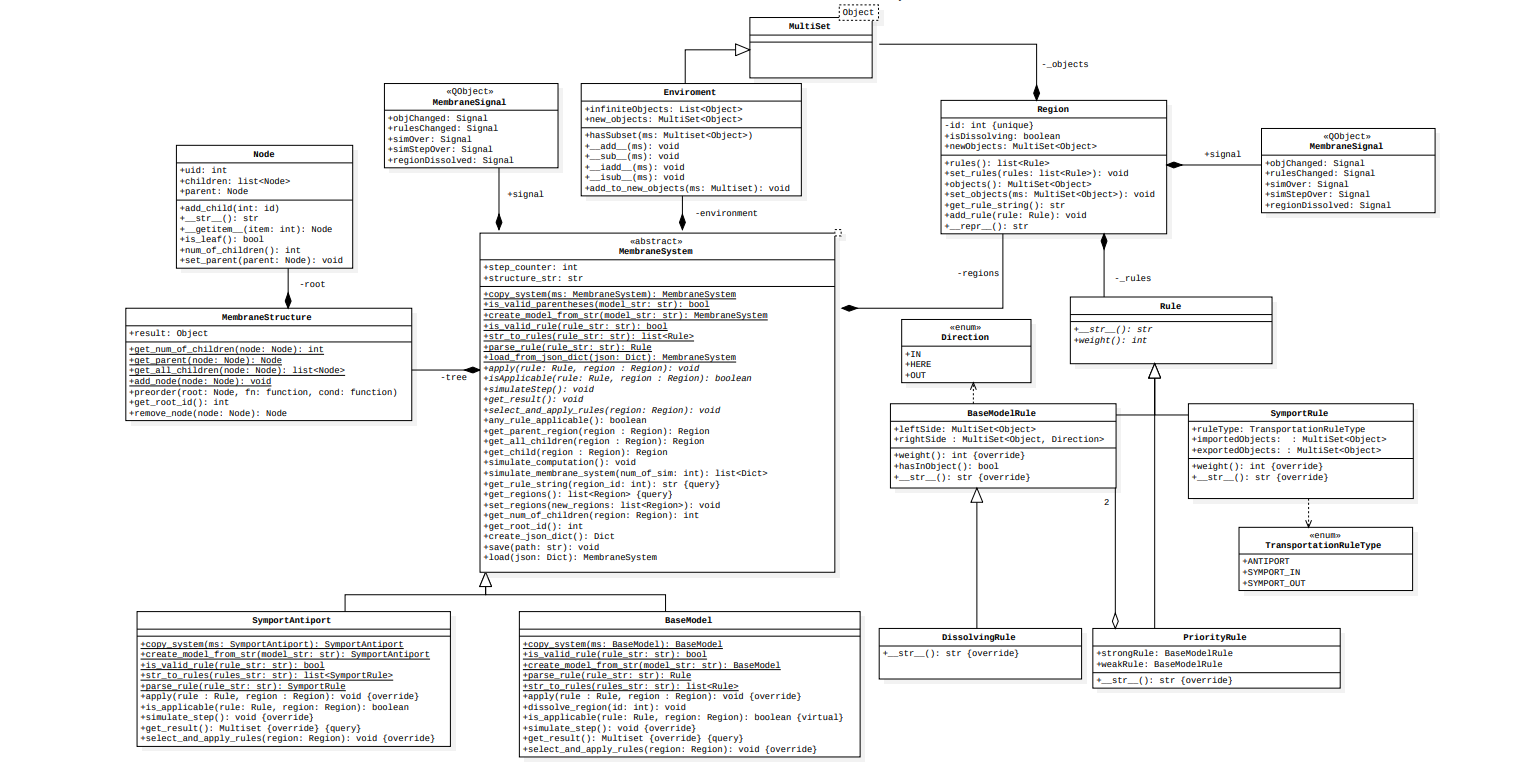
\includegraphics{model_uml.png}
	\caption{A főablak az alkalmazás megnyitásakor}
	\label{fig:main_window}
\end{figure}





\section{Forráskódok}

Nulla sodales purus id mi consequat, eu venenatis odio pharetra. Cras a arcu quam. Suspendisse augue risus, pulvinar a turpis et, commodo aliquet turpis. Nulla aliquam scelerisque mi eget pharetra. Mauris sed posuere elit, ac lobortis metus. Proin lacinia sit amet diam sed auctor. Nam viverra orci id sapien sollicitudin, a aliquam lacus suscipit. Quisque ac tincidunt leo \ref{src:cpp}. és \ref{src:csharp}.~forráskód:

\lstset{caption={Hello World in C++}, label=src:cpp}
\begin{lstlisting}[language={C++}]
#include <stdio>

int main() 
{
	int c;
	std::cout << "Hello World!" << std::endl;

	std::cout << "Press any key to exit." << std::endl;
	std::cin >> c;
	
	return 0;
}
\end{lstlisting}

\lstset{caption={Hello World in C\#}, label=src:csharp}
\begin{lstlisting}[language={[Sharp]C}]
using System;
namespace HelloWorld
{
	class Hello 
	{
		static void Main() 
		{
			Console.WriteLine("Hello World!");
			
			Console.WriteLine("Press any key to exit.");
			Console.ReadKey();
		}
	}
}
\end{lstlisting}

\subsection{Algoritmusok}

Az \ref{alg:ibb}.~algoritmus egy általános elágazás és korlátozás algoritmust (\emph{Branch and Bound algorithm}) mutat be. A \ref{step:selrule}.~lépésben egy megfelelő kiválasztási szabályt kell alkalmazni.
Példa forrása: \href{https://www.inf.u-szeged.hu/actacybernetica/}{Acta Cybernetica (ez egy hiperlink)}.

\begin{algorithm}[H]
\caption{A general interval B\&B algorithm}
\label{alg:ibb}
\textbf{\underline{Funct}} IBB($S,f$)
\begin{algorithmic}[1] % sorszámok megjelenítése minden n. sor előtt, most n = 1
\State Set the working list ${\cal L}_W$ := $\{S\}$ and the final list ${\cal L}_Q$ := $\{\}$
\While{( ${\cal L}_W \neq \emptyset$ )} \label{alg:igoend}
	\State Select an interval $X$ from ${\cal L}_W$ \label{step:selrule}\Comment{Selection rule}
	\State Compute $lbf(X)$ \Comment{Bounding rule}
	\If{$X$ cannot be eliminated} \Comment{Elimination rule}
		\State Divide $X$ into $X^j,\ j=1,\dots, p$, subintervals   \Comment{Division rule}
		\For{$j=1,\ldots,p$}
			\If{$X^j$ satisfies the termination criterion} \Comment{Termination rule}
				\State Store $X^j$ in ${\cal L}_W$
			\Else
				\State Store $X^j$ in ${\cal L}_W$
			\EndIf
		\EndFor
	\EndIf
\EndWhile
\State \textbf{return} ${\cal L}_Q$
\end{algorithmic}
\end{algorithm}

\cleardoublepage

\chapter{Összegzés}
\label{ch:sum}
A megvalósított szoftver a membránrendszerek alapmodelljének és a szimport-antiport rendszerek tetszőleges példányát képes a felhasználó által megadott konfiguráció segítségével megalkotni, majd szimulálni.  A szimulálás során biztosítja a nemdeterminisztikusságot, amelynek szemléltetésére a membránrendszer aktuális állapotából kiinduló párhuzamos számítások esetén egy összegzést készít a felhasználó számára.A lépésenkénti futtatás során is tanúja lehet a felhasználó a rendszer véletlenszerű fejlődésének.
A membránrendszerekkel való ismerkedés és az alkalmazás teljes funkcionalitásának elsajátítása céljából egy használati útmutató is található az alkalmazásban, amely elegendő információt nyújt az előbb említett mindkét területen való kezdeti útbaigazításhoz. Az absztrakt modellhez és a természet által inspirált struktúrához a membránrendszer a grafikus felületen vizuálisan jelenik meg, így az a használat során egy felhasználóbarát és intuitív interfészt biztosít a mögöttes reprezentáció manipulálásához. Így a matematikailag nehezen leírható konfigurációk és konfigurációátmenet-sorozatok egyszerűen és szemléletesen mutathatók be, ezáltal könnyebb megértést adva a definíciókhoz.

A modellezés során kulcsfontosságú metódusok az alkalmazás tervezési fázisában majdnem teljes mértékben elkészültek, ám az eredeti modell megvalósítása után felbukkant pár kezeletlen eset, illetve  módosítandó algoritmus. Ezen hibák kiszűrésében és a helyes implementáció megalkotásában központi szerepet játszottak az egyes osztályokhoz és funkciókhoz tartozó egységtesztek.

Az alkalmazás továbfejlesztésére számos lehetőség adott, amelyek implementálását elősegíti a bővíthetőségre és karbantarthatóságra tekintettel megalkotott modell architektúra. Az egyik legérdekesebb kiegészítése a programnak az aktív P-rendszerek szimulálásának támogatása, amely esetén a régiók töltéssel rendelkeznek és bizonyos szabályok segítségével akár osztódni is képesek.
\cleardoublepage

% Appendices (optional) - useful for detailed information in long tables, many and/or large figures, etc.
\appendix
\chapter{Szimulációs eredmények}
\label{appx:simulation}

Lorem ipsum dolor sit amet, consectetur adipiscing elit. Pellentesque facilisis in nibh auctor molestie. Donec porta tortor mauris. Cras in lacus in purus ultricies blandit. Proin dolor erat, pulvinar posuere orci ac, eleifend ultrices libero. Donec elementum et elit a ullamcorper. Nunc tincidunt, lorem et consectetur tincidunt, ante sapien scelerisque neque, eu bibendum felis augue non est. Maecenas nibh arcu, ultrices et libero id, egestas tempus mauris. Etiam iaculis dui nec augue venenatis, fermentum posuere justo congue. Nullam sit amet porttitor sem, at porttitor augue. Proin bibendum justo at ornare efficitur. Donec tempor turpis ligula, vitae viverra felis finibus eu. Curabitur sed libero ac urna condimentum gravida. Donec tincidunt neque sit amet neque luctus auctor vel eget tortor. Integer dignissim, urna ut lobortis volutpat, justo nunc convallis diam, sit amet vulputate erat eros eu velit. Mauris porttitor dictum ante, commodo facilisis ex suscipit sed.

Sed egestas dapibus nisl, vitae fringilla justo. Donec eget condimentum lectus, molestie mattis nunc. Nulla ac faucibus dui. Nullam a congue erat. Ut accumsan sed sapien quis porttitor. Ut pellentesque, est ac posuere pulvinar, tortor mauris fermentum nulla, sit amet fringilla sapien sapien quis velit. Integer accumsan placerat lorem, eu aliquam urna consectetur eget. In ligula orci, dignissim sed consequat ac, porta at metus. Phasellus ipsum tellus, molestie ut lacus tempus, rutrum convallis elit. Suspendisse arcu orci, luctus vitae ultricies quis, bibendum sed elit. Vivamus at sem maximus leo placerat gravida semper vel mi. Etiam hendrerit sed massa ut lacinia. Morbi varius libero odio, sit amet auctor nunc interdum sit amet.

Aenean non mauris accumsan, rutrum nisi non, porttitor enim. Maecenas vel tortor ex. Proin vulputate tellus luctus egestas fermentum. In nec lobortis risus, sit amet tincidunt purus. Nam id turpis venenatis, vehicula nisl sed, ultricies nibh. Suspendisse in libero nec nisi tempor vestibulum. Integer eu dui congue enim venenatis lobortis. Donec sed elementum nunc. Nulla facilisi. Maecenas cursus id lorem et finibus. Sed fermentum molestie erat, nec tempor lorem facilisis cursus. In vel nulla id orci fringilla facilisis. Cras non bibendum odio, ac vestibulum ex. Donec turpis urna, tincidunt ut mi eu, finibus facilisis lorem. Praesent posuere nisl nec dui accumsan, sed interdum odio malesuada.
\cleardoublepage

% Bibliography (mandatory)
\phantomsection
\addcontentsline{toc}{chapter}{\biblabel}
\printbibliography[title=\biblabel]
\cleardoublepage

% List of figures (optional) - useful over 3-5 figures
\phantomsection
\addcontentsline{toc}{chapter}{\lstfigurelabel}
\listoffigures
\cleardoublepage

% List of tables (optional) - useful over 3-5 tables
\phantomsection
\addcontentsline{toc}{chapter}{\lsttablelabel}
\listoftables
\cleardoublepage

% List of algorithms (optional) - useful over 3-5 algorithms
\phantomsection
\addcontentsline{toc}{chapter}{\lstalgorithmlabel}
\listofalgorithms
\cleardoublepage

% List of codes (optional) - useful over 3-5 code samples
\phantomsection
\addcontentsline{toc}{chapter}{\lstcodelabel}
\lstlistoflistings
\cleardoublepage

% List of symbols (optional)
%\printnomenclature

\end{document}